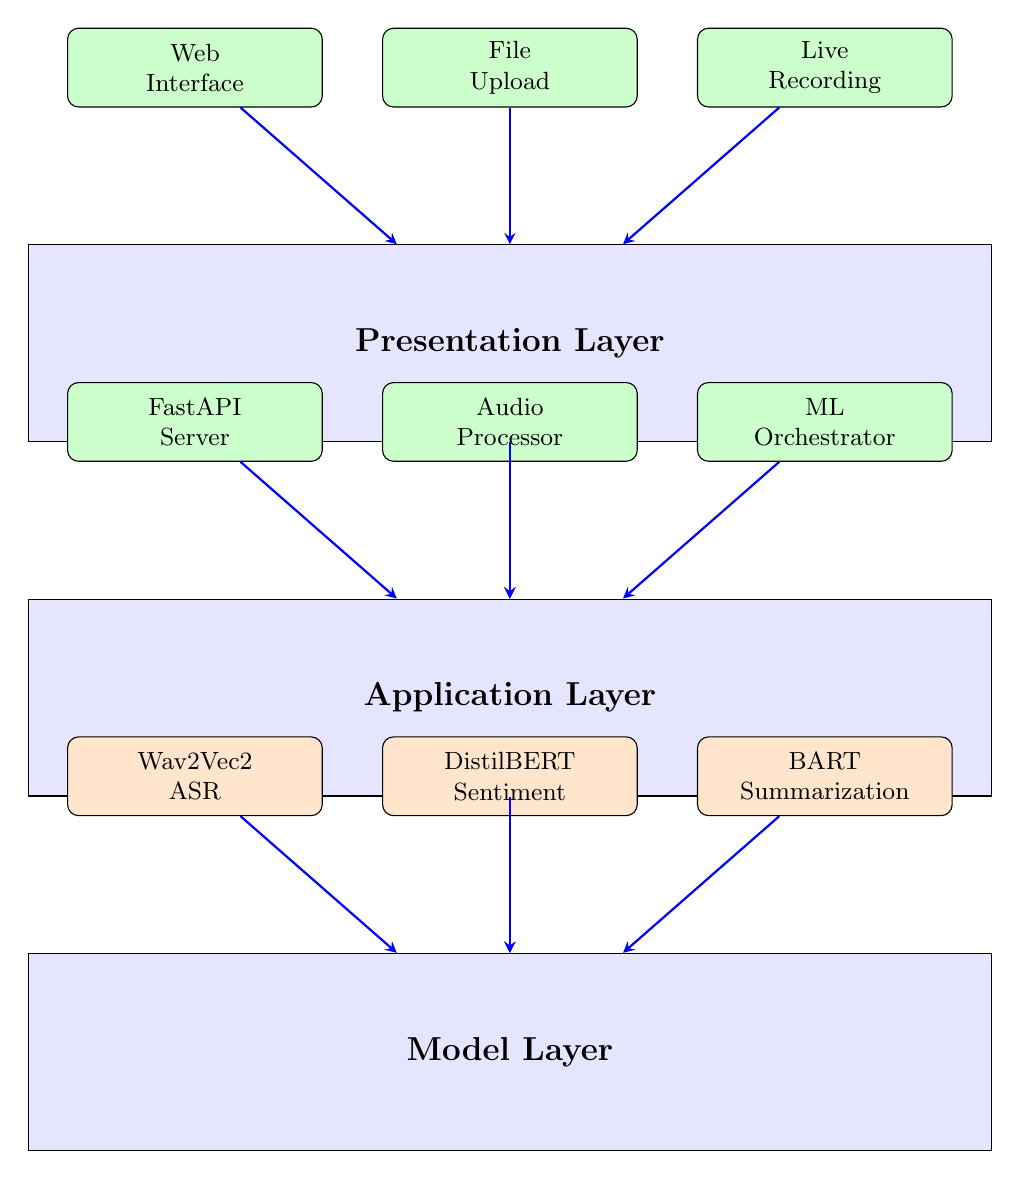
\begin{tikzpicture}[
    node distance=2.5cm,
    layer/.style={rectangle, draw, fill=blue!10, text width=12cm, minimum height=2.5cm, align=center, font=\large\bfseries},
    component/.style={rectangle, draw, fill=green!20, text width=3cm, text centered, rounded corners, minimum height=1cm, font=\small},
    model/.style={rectangle, draw, fill=orange!20, text width=3cm, text centered, rounded corners, minimum height=1cm, font=\small},
    arrow/.style={->, >=stealth, thick}
]

% Layers
\node[layer] (presentation) {Presentation Layer};
\node[layer, below of=presentation, yshift=-2cm] (application) {Application Layer};
\node[layer, below of=application, yshift=-2cm] (model_layer) {Model Layer};

% Presentation components
\node[component, above of=presentation, yshift=1cm, xshift=-4cm] (web) {Web\\Interface};
\node[component, above of=presentation, yshift=1cm, xshift=0cm] (upload) {File\\Upload};
\node[component, above of=presentation, yshift=1cm, xshift=4cm] (record) {Live\\Recording};

% Application components
\node[component, above of=application, yshift=1cm, xshift=-4cm] (api) {FastAPI\\Server};
\node[component, above of=application, yshift=1cm, xshift=0cm] (audio_proc) {Audio\\Processor};
\node[component, above of=application, yshift=1cm, xshift=4cm] (orchestrator) {ML\\Orchestrator};

% Model components
\node[model, above of=model_layer, yshift=1cm, xshift=-4cm] (asr) {Wav2Vec2\\ASR};
\node[model, above of=model_layer, yshift=1cm, xshift=0cm] (sentiment) {DistilBERT\\Sentiment};
\node[model, above of=model_layer, yshift=1cm, xshift=4cm] (summary) {BART\\Summarization};

% Vertical arrows between layers
\draw[arrow, blue] (web) -- (presentation);
\draw[arrow, blue] (upload) -- (presentation);
\draw[arrow, blue] (record) -- (presentation);

\draw[arrow, blue] (presentation) -- (application);

\draw[arrow, blue] (api) -- (application);
\draw[arrow, blue] (audio_proc) -- (application);
\draw[arrow, blue] (orchestrator) -- (application);

\draw[arrow, blue] (application) -- (model_layer);

\draw[arrow, blue] (asr) -- (model_layer);
\draw[arrow, blue] (sentiment) -- (model_layer);
\draw[arrow, blue] (summary) -- (model_layer);

\end{tikzpicture}
